\chapter*{Avant propos}
%\thispagestyle{empty}
%\section*{Histoire}
%\setlength{\parindent}{20px}
L'histoire de la vision par ordinateur n'a pas pu enregistrer une évolution considérable qu'après l'effervescence des techniques de l'intelligence artificielle. Les recherches scientifiques ont profité de la quantité massive des données disponible pour développer des modèles mathématiques capables d'analyser ou de traiter un contenu numérique sans pour autant avoir recours aux méthodes classiques. \`A titre d'exemple, imaginons le nombre de personnes nécessaire pour contrôler et approuver les publications sur une plate-forme comme YouTube où, pour chaque minute, plus de 500 heures de vidéos sont mises en ligne \needRef. Une simple estimation montre qu'il faut plus de 225000 personnes pour les visualiser.

Les premiers algorithmes dans le domaine de l'intelligence artificielle exploitent des données structurées, qualitatives ou quantitatives. Par exemple, dans le cas de prédiction des sujets potentiellement diabétiques, les informations telles que l'âge, le genre, la glycémie peuvent être récoltées avec d'autres indicateurs pour former une base sur l'état de santé d'une population donnée. Les informations relatives à un sujet sont conventionnellement appelées observation. Comment pouvons-nous prédire, pour un nouveau sujet, qu'il présente des risques de diabète ? Certains domaines sont sensibles à l'échec.

Ces observations modélisent, avec un certain niveau d'abstraction, le monde réel. Ce qui renforce le doute qu'elles suivent une certaine logique ou qu'elles cachent des corrélations ou des phénomènes plus complexes. Le but est alors de dévoiler ces dépendances sous forme d'un modèle mathématique capable de correspondre chaque observation à un résultat attendu. \`A ce stade, les statisticiens peuvent revendiquer le droit qu'ils sont des problèmes d'ordre statistique. Toutefois, cette nuance disparaîtra à fur et à mesure que les objectifs et les problèmes se diversifient et se complexifient.

Les réseaux de neurones n'ont pas seulement mis fin à ce débat mais ils ont encore poussé les limites de IA pour enfin parler de l'apprentissage automatique. Sans vouloir tomber dans un abus de langage, laissons momentanément à côté les définitions. Le réel apport de cette technologie par rapport au machine learning classique est que le choix des variables pertinentes qui agissent sur la qualité de la prédiction ne sont pas la tâche du "data-scientist" mais plutôt la machine. Cette configuration automatique, appelée feature-selection, d'une part donne des résultats plus pertinants et d'autre part élargie le domaine d'application. En effet, on n'est plus sous la contrainte d'étudier manuellement l'influence de chaque variable pour arriver au meilleur modèle. En d'autres termes le nombre des variables ne compte plus parmi les obstacles. Ceci est clairement visible dans les problèmes de reconnaissance, par exemple. L'extraction des caractéristiques des formes à reconnaître n'est plus confiée au développeur. C'est plutôt la machine qui s'en charge. Certe une préparation préalable des données peut être exigée, mais l'extraction des caractéristiques reste automatisée.

Nous y sommes maintenant dans le Deep learning, dans les réseaux de neurones à convolution. Cette technologie a conservé l'architecture des réseaux de neurones, et a ajouté des transformations sous forme de couches dites à convolution. Avec cette réadaptation, le réseau devient capable d'extraire les informations susceptibles d'être des caractéristiques pour les employer par la suite comme "features" d'un exemple.


\begin{figure}[H]
\centering
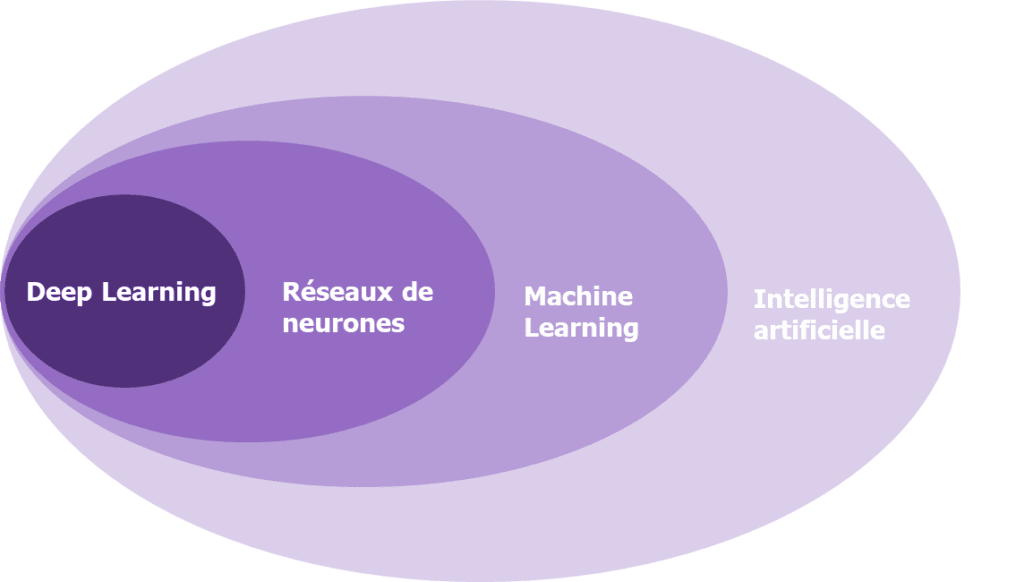
\includegraphics[width=12cm]{figures/AP/image-1-1.png}
\caption{Domaines de l'intelligence artificielle}
\end{figure}
